% Niveau :      PCSI *
% Discipline :  Chimie Orga
% Mots clés :   Stéréochimie

\begin{exercise}{\'Equilibre céto-énolique et RMN}{2}{PCSI}
{Chimie organique I,Spectroscopie,RMN,Tautomérie}{bermu}

\begin{questions}
\questioncours RMN du proton $^{1}$H. Réalisation d'un spectre, principe de fonctionnement. Déplacement chimique $\delta$ : influence de l'environnement chimique et du solvant.

\begin{figure}[H]
    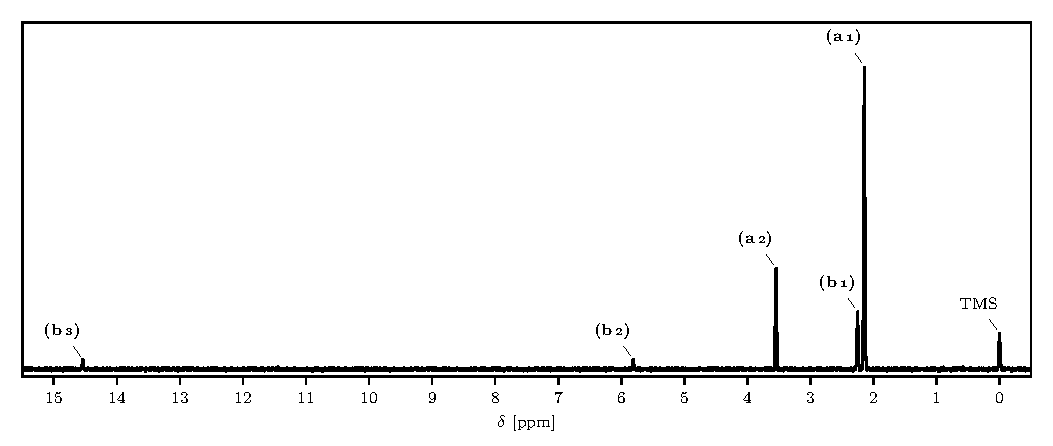
\includegraphics[width=\linewidth]{chimiePC/orga/keto1.pdf},
    \centering
    \begin{tabularx}{.7\linewidth}{c|l|CcCCCC}
        & & \multicolumn{6}{l}{\textbf{Intégration} pour différents solvants} \\
        & $\boldsymbol{\delta}$ \textbf{[ppm]} & $\mathrm{D_2O}$ & $\mathrm{DMSO}$-$d_6$ & $\mathrm{D_3COD}$ & Pur & $\mathrm{DCC\ell_3}$ & $\mathrm{C_6D_{12}}$ \\ \hline\hline
        \textbf{(a{\tiny\,1})} & $2.14$ & $1.00$ & $0.61$ & $0.35$ & $0.23$ & $0.05$ & $0.03$ \\
        \textbf{(a{\tiny\,2})} & $3.54$ & $0.33$ & $0.20$ & $0.12$ & $0.08$ & $0.02$ & $0.01$ \\
        \textbf{(b{\tiny\,1})} & $2.25$ & $0.19$ & $1.00$ & $1.00$ & $1.00$ & $1.00$ & $1.00$ \\
        \textbf{(b{\tiny\,2})} & $5.81$ & $0.03$ & $0.17$ & $0.17$ & $0.17$ & $0.17$ & $0.17$ \\
        \textbf{(b{\tiny\,3})} & $14.54$ & $0.03$ & $0.17$ & $0.17$ & $0.17$ & $0.17$ & $0.17$ \\\hline
    \end{tabularx}
    \caption{Spectres RMN $^{1}$H à 600 Hz du composé $\mathrm{C_5H_8O_2}$ réalisés dans différents solvants. \newline Le spectre tracé est effectué dans $\mathrm{D_2O}$.}
\end{figure}

\question \'Etant donné le spectre RMN ci-dessus, retrouver la structure du composé \textbf{A} de formule brute $\mathrm{C_5H_8O_2}$. On ne prendra en compte que les pics numérotés $\textbf{(a\,i)}$.

\question La présence du second groupe de pics, notés $\textbf{(b\,i)}$, est due à un second composé \textbf{B} en équilibre avec \textbf{A}, $\textbf{A} \xrightleftharpoons{} \textbf{B}.$ \\
Quelle est la structure de \textbf{B} ?

\question Commenter le déplacement chimique du pic \textbf{(b{\tiny\,3})}. Connaissez-vous d'autres fonctions qui ont un déplacement aussi élevé ? Pourquoi utiliser des solvants deutérés ?

\question \`A partir de la table d'intégration, donnez la fraction molaire $x_\textbf{A}$ de \textbf{A} pour chaque solvant.

\question Commenter l'évolution de $x_\textbf{A}$ dans chaque sovlant.
\end{questions}

\plusloin Discuter des constantes de vitesse de la réaction $\textbf{A} \xrightleftharpoons{} \textbf{B}$ par rapport à la résolution en fréquence de l'appareil.

\end{exercise}